% IMT-342 Robótica — Hito 2
% Basado en la plantilla oficial: Semana_10/hito_2/hito_2_ieee_template.tex
% Actualizado: 19 de octubre de 2026
% ANTES DE ENTREGAR: completar autores y datos de las poses oficiales,
% si el docente las proporciona. No presentar la pose de autocontrol como oficial.
\documentclass[conference]{IEEEtran}

\usepackage[T1]{fontenc}
\usepackage[utf8]{inputenc}
\usepackage[spanish,es-noshorthands]{babel}
\usepackage{amsmath,amssymb,bm}
\usepackage{graphicx}
\usepackage{cite}
\usepackage{booktabs}
\usepackage{array}
\usepackage{url}

\begin{document}

\title{Integración de Modelos Cinemáticos, Diferenciales y Dinámicos para Manipuladores: Hito 2 del ABB IRB 120}

% DATOS PENDIENTES: sustituir nombres, sede y correos reales del equipo.
% Si son más de dos integrantes, agregar bloques IEEEauthorblockN / IEEEauthorblockA.
\author{
\IEEEauthorblockN{Roberth Williams Ruiz Condori}
\IEEEauthorblockA{\textit{Ingeniería Mecatrónica}\\
\textit{Universidad Católica Boliviana}\\
Bolivia\\
roberth.ruiz@ucb.edu.bo}
\and
\IEEEauthorblockN{Mario Alberto Nina Gallo}
\IEEEauthorblockA{\textit{Ingeniería Mecatrónica}\\
\textit{Universidad Católica Boliviana}\\
Bolivia\\
mario.nina@ucb.edu.bo}
}

\maketitle

\begin{abstract}
Se implementó y validó un flujo computacional para el manipulador ABB IRB 120 de seis articulaciones revolutas que enlaza cinemática inversa analítica de Pieper, verificación por cinemática directa, selección de configuraciones según límites articulares, planificación LSPB y análisis diferencial mediante el Jacobiano geométrico. Además, se estudió una singularidad de muñeca y se evaluó un modelo dinámico pedagógico independiente de un grado de libertad (1R), alimentado por una trayectoria LSPB. Para una pose de autocontrol generada mediante cinemática directa se obtuvieron ocho ramas matemáticas, de las cuales dos ramas poseyeron representaciones dentro de los límites nominales considerados. Los errores de reconstrucción de posición fueron del orden de $10^{-16}$\,m. En la singularidad de muñeca $q_5=0$ se observó reducción de rango de seis a cinco, mientras que el ejemplo dinámico del docente produjo $\tau(2.5\,\mathrm{s})=4.429791$\,N\,m. El cuaderno integrador se ejecutó sin errores y la batería de regresión reportó 71 pruebas satisfactorias. Los casos de autocontrol no sustituyen las poses objetivo que deba asignar el docente; asimismo, el modelo 1R no predice torques reales de los actuadores ABB.
\end{abstract}

\begin{IEEEkeywords}
ABB IRB 120, cinemática inversa, Pieper, Denavit--Hartenberg, LSPB, Jacobiano geométrico, singularidades, dinámica reducida.
\end{IEEEkeywords}

\section{Introducción}
La planificación de movimiento de un manipulador exige conectar la geometría del espacio cartesiano con la configuración articular y su evolución temporal. La cinemática inversa determina las posiciones articulares compatibles con una pose objetivo; la cinemática directa (FK) permite comprobarlas. Posteriormente, la trayectoria LSPB prescribe posiciones, velocidades y aceleraciones, mientras que el Jacobiano relaciona velocidades articulares y cartesianas. El análisis de singularidades identifica configuraciones en las que se pierde movilidad instantánea \cite{siciliano}.

El Hito 2 de IMT-342 requiere integrar estos bloques en un Notebook reproducible e incluir un cálculo dinámico reducido 1R, junto con evidencias y un informe IEEE \cite{guiaH2,rubricaH2}. En este documento se presentan las formulaciones utilizadas, el caso de autocontrol efectivamente comprobado, los resultados cuantitativos y sus limitaciones. Las poses utilizadas en esta versión \emph{no fueron proporcionadas como consignas oficiales}; el pipeline queda preparado para recibirlas cuando estén disponibles.

\section{Metodología}
\subsection{Modelo geométrico y convenciones}
El modelo cinemático del ABB IRB 120 consta de seis juntas revolutas. Se adoptó la convención Denavit--Hartenberg (D--H) estándar, ya validada durante el Hito 1, con distancias en metros y ángulos en radianes. Los parámetros utilizados se presentan en la Tabla~\ref{tab:dh}. Los datos geométricos y los límites nominales se contrastaron con la documentación del fabricante \cite{abbSpec,abbManual}; la asignación de marcos D--H y el desplazamiento en la segunda coordenada corresponden al modelo académico del equipo.

\begin{table}[!t]
\caption{Parámetros D--H estándar del modelo académico del IRB 120}
\label{tab:dh}
\centering
\footnotesize
\setlength{\tabcolsep}{4pt}
\begin{tabular}{ccccc}
\toprule
$i$ & $\theta_i$ & $d_i$ [m] & $a_i$ [m] & $\alpha_i$ \\
\midrule
1 & $q_1$ & 0.290 & 0 & $-\pi/2$ \\
2 & $q_2-\pi/2$ & 0 & 0.270 & $0$ \\
3 & $q_3$ & 0 & 0.070 & $-\pi/2$ \\
4 & $q_4$ & 0.302 & 0 & $+\pi/2$ \\
5 & $q_5$ & 0 & 0 & $-\pi/2$ \\
6 & $q_6$ & 0.072 & 0 & $0$ \\
\bottomrule
\end{tabular}
\end{table}

La transformación homogénea se construye mediante
\begin{equation}
{}^{0}\!T_6(\bm q)=\prod_{i=1}^{6} {}^{i-1}\!T_i(\theta_i,d_i,a_i,\alpha_i).
\label{eq:fk}
\end{equation}
En el experimento principal se emplea la brida $\{6\}$ como efector; no se confunde con el TCP académico, cuyo desplazamiento adicional sobre $z_6$ es de $0.120$\,m.

\subsection{Cinemática inversa de Pieper y validación FK}
Para evitar atribuir al docente una pose no entregada, se generó una consigna verificable a partir de la configuración elegida por el equipo:
\begin{equation}
\bm q_{\mathrm{ref}}=\begin{bmatrix}
0.30&-0.20&0.10&0.20&-0.40&0.50
\end{bmatrix}^{\!T}\;\mathrm{rad}.
\label{eq:qref}
\end{equation}
La pose objetivo se definió como $T_d={}^{0}\!T_6(\bm q_{\mathrm{ref}})$. Con el desacoplamiento geométrico de Pieper, el centro de muñeca de la brida se determina por
\begin{equation}
\bm p_{wc}=\bm p_d-d_6 R_d\hat{\bm z},\qquad d_6=0.072\,\mathrm m,
\label{eq:wc}
\end{equation}
y la orientación residual mediante
\begin{equation}
R_3^6=(R_0^3)^T R_d.
\label{eq:residual}
\end{equation}
Se enumeran las ramas geométricas de brazo y muñeca utilizando $\operatorname{atan2}$ para conservar cuadrantes. Las configuraciones que resuelven la IK se filtran posteriormente según los límites nominales ABB; esta comprobación es independiente de la existencia matemática de cada rama.

Cada solución $\bm q^{(k)}$ se verifica reinyectándola en FK. Se utilizan los errores
\begin{align}
e_p^{(k)}&=\left\|\bm p(\bm q^{(k)})-\bm p_d\right\|_2,\label{eq:ep}\\
e_R^{(k)}&=\cos^{-1}\!\left(\operatorname{clip}\!\left[\frac{\operatorname{tr}(R_d^T R_k)-1}{2},-1,1\right]\right),\label{eq:er}
\end{align}
con umbrales de autocontrol $e_p<10^{-7}$\,m y $e_R<10^{-6}$\,rad. Para escoger la solución de movimiento se minimiza $\sum_i w_i(q_i-q_{i,0})^2$, usando pesos unitarios y $\bm q_0=\bm0$; también se consideran representaciones equivalentes permitidas de J6 separadas por $2\pi$.

\subsection{Trayectorias articulares LSPB}
El planificador interpola desde $\bm q_0$ hasta la solución seleccionada con reposo en ambos extremos. Para cada articulación se utiliza una aceleración de magnitud $a_i$ y un tiempo de mezcla $t_{c,i}$ que satisface
\begin{equation}
|q_{f,i}-q_{0,i}|=a_i t_{c,i}(t_f-t_{c,i}).
\label{eq:tc}
\end{equation}
El perfil posee una fase de aceleración uniforme, una fase de velocidad constante $v_{c,i}=\operatorname{sgn}(\Delta q_i)a_i t_{c,i}$ y otra de frenado, de manera que $q_i(t)$ y $\dot q_i(t)$ sean continuas. La aceleración $\ddot q_i(t)$ puede presentar saltos ideales en las transiciones. Para el caso 6R se adoptaron $t_f=8$\,s y $a_i=1$\,rad/s$^2$: son elecciones de planificación académica, \emph{no} aceleraciones certificadas por ABB. El software contrasta posiciones y velocidades con los rangos nominales considerados \cite{abbSpec}.

\subsection{Jacobiano geométrico y velocidades}
Para juntas revolutas, cada columna del Jacobiano de la brida, expresado en la base, está dada por
\begin{equation}
J_i=\begin{bmatrix}
\bm z_{i-1}\times(\bm p_e-\bm o_{i-1})\\
\bm z_{i-1}
\end{bmatrix},\qquad
\mathcal V_6=J(\bm q)\dot{\bm q}.
\label{eq:jac}
\end{equation}
Las tres primeras filas representan velocidad lineal y las tres últimas velocidad angular. La primera columna se contrastó manualmente, de forma independiente del módulo, mediante $\bm z_0=[0,0,1]^T$ y $\bm o_0=\bm0$; la comparación con la implementación fue satisfactoria.

\subsection{Experimento independiente de singularidad}
Se fijaron $q_1=0.30$, $q_2=-0.35$, $q_3=0.25$, $q_4=0.40$ y $q_6=-0.60$\,rad, mientras $q_5$ se aproximó a cero desde $0.2$\,rad. La pérdida de rango se determinó mediante descomposición en valores singulares. Para comparar componentes lineales y angulares se utilizó, como convención del equipo, una longitud de referencia $L=1$\,m:
\begin{equation}
J_n=\operatorname{diag}(L^{-1}I_3,I_3)J.
\label{eq:jn}
\end{equation}
El criterio numérico de rango empleó tolerancia relativa $10^{-9}$. Una misma consigna cartesiana, elegida en la dirección instantáneamente perdida de la configuración singular, permitió observar el crecimiento de $\|\dot{\bm q}\|$ en las posturas regulares cercanas. En la postura singular no se invirtió la matriz. Las velocidades resultantes son \emph{diagnósticos matemáticos}, no consignas seguras para los motores \cite{rubricaH2}.

\subsection{Dinámica reducida 1R}
Se utilizó \emph{separadamente} el modelo pedagógico de un grado de libertad especificado por el docente \cite{guiaH2,practicaS10}:
\begin{equation}
\tau(t)=\underbrace{J_{1R}\ddot q(t)}_{\tau_I(t)}+
\underbrace{mg\ell_c\sin q(t)}_{\tau_g(t)},
\label{eq:tau}
\end{equation}
donde $J_{1R}$ es la inercia escalar constante del ejemplo, distinta del Jacobiano geométrico $J(\bm q)$. Se adoptaron los valores didácticos $J_{1R}=0.25$\,kg\,m$^2$, $m=1$\,kg, $\ell_c=0.5$\,m y $g=9.81$\,m/s$^2$, alimentando la ecuación con un LSPB 1R que va de $0$ a $2$\,rad en $3$\,s, con $a=1$\,rad/s$^2$. En este modelo particular de inercia constante no aparece un término independiente de Coriolis. El cálculo no representa el acoplamiento dinámico ni el torque físico de los seis actuadores del ABB IRB 120.

\section{Resultados clave}
\subsection{Ramas de Pieper y reconstrucción geométrica}
La matriz de referencia calculada mediante FK fue
\begin{equation}
T_d\simeq
\begin{bmatrix}
-0.205011 & 0.463620 & 0.861990 & 0.291212\\
-0.723347 &-0.665055 & 0.185662 & 0.084252\\
 0.659348 &-0.585455 & 0.471702 & 0.688380\\
 0 &0&0&1
\end{bmatrix}.
\label{eq:target}
\end{equation}
Los elementos rotacionales de \eqref{eq:target} se muestran redondeados; el programa utiliza la matriz completa sin redondear. Se hallaron ocho ramas analíticas regulares y se validaron todas mediante FK. La Tabla~\ref{tab:ramas} resume el filtrado. Dos ramas diferentes cumplen los rangos nominales en sus representantes admitidos; al considerar vueltas equivalentes de J6 resultan cinco representaciones admisibles en total. No se deben confundir estas cinco representaciones con cinco soluciones geométricas independientes.

\begin{table}[!t]
\caption{Ocho ramas de Pieper y admisibilidad nominal ABB}
\label{tab:ramas}
\centering
\footnotesize
\setlength{\tabcolsep}{4pt}
\begin{tabular}{ccccc}
\toprule
Rama & Base & Codo & Muñeca & Admisible \\
\midrule
1 & directa & $+$ & $+$ & No \\
2 & directa & $+$ & $-$ & Sí \\
3 & directa & $-$ & $+$ & No \\
4 & directa & $-$ & $-$ & No \\
5 & opuesta & $+$ & $+$ & No \\
6 & opuesta & $+$ & $-$ & Sí \\
7 & opuesta & $-$ & $+$ & No \\
8 & opuesta & $-$ & $-$ & No \\
\bottomrule
\end{tabular}
\end{table}

El mayor error posicional reconstruido entre las ocho ramas fue aproximadamente $1.8\times10^{-16}$\,m; el error angular quedó dentro del umbral de $10^{-6}$\,rad. Se eligió
\begin{equation}
\bm q_f=[0.30,-0.20,0.10,0.20,-0.40,0.50]^T\;\mathrm{rad},
\end{equation}
correspondiente a base directa, codo $+$ y muñeca $-$, con costo articular de $0.59$\,rad$^2$ para pesos unitarios y referencia inicial nula.

\subsection{Trayectoria LSPB y mapeo diferencial}
La Fig.~\ref{fig:lspb} muestra las seis trayectorias articulares con posición y velocidad continuas, y saltos de aceleración en los puntos de mezcla. Los valores $t_{c,i}$ estuvieron aproximadamente entre $0.0125$ y $0.0630$\,s, de acuerdo con la distancia articular de cada eje. Se verificó $\bm q(0)=\bm q_0$, $\bm q(8)=\bm q_f$ y $\dot{\bm q}(0)=\dot{\bm q}(8)=\bm0$. El cálculo de $J(\bm q(t))\dot{\bm q}(t)$ también produjo velocidad de brida nula en ambos extremos, como corresponde a la condición de reposo.

\begin{figure}[!t]
\centering
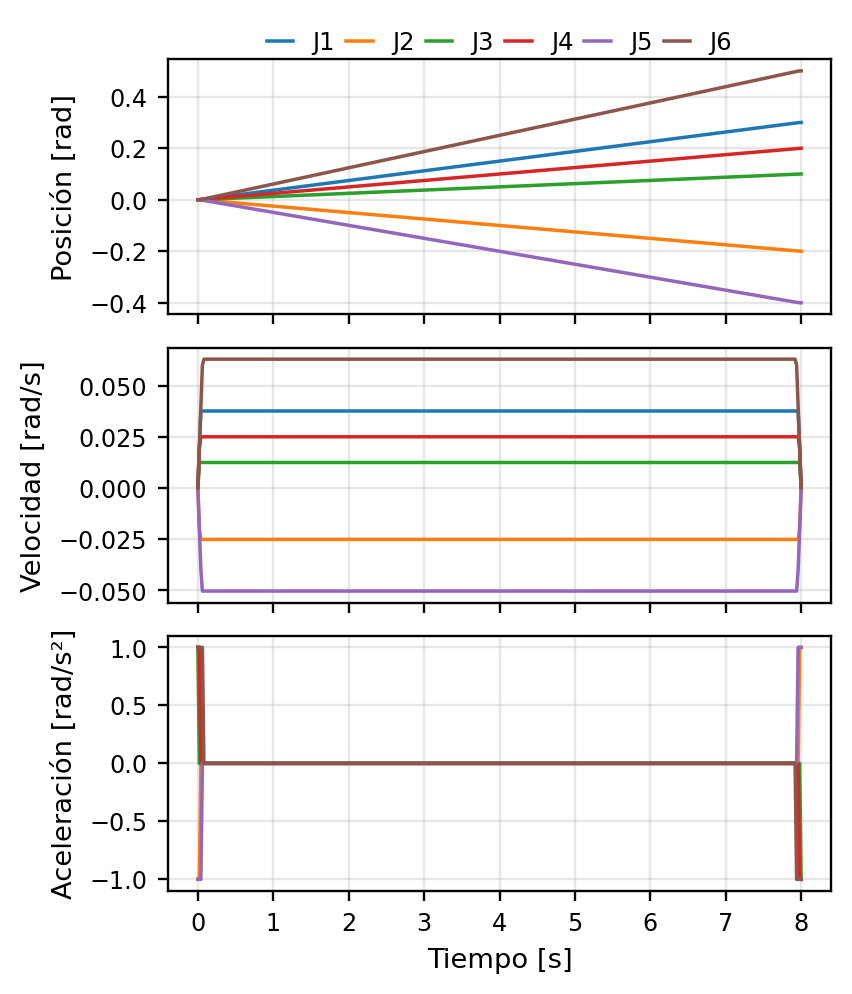
\includegraphics[width=0.91\columnwidth]{figuras/lspb_6r.png}
\caption{Perfiles articulares LSPB de seis juntas para el caso de autocontrol: posición, velocidad y aceleración. Duración total $8$\,s; aceleraciones académicas de $1$\,rad/s$^2$ por junta.}
\label{fig:lspb}
\end{figure}

\subsection{Pérdida de rango en la muñeca}
La Fig.~\ref{fig:sing} exhibe la transición de rango seis a cinco en $q_5=0$. En esta posición los ejes de las juntas J4 y J6 se alinean, por lo que el robot pierde una dirección independiente de velocidad cartesiana instantánea. Para una consigna cartesiana fija se observó $\|\dot{\bm q}\|\simeq0.353$\,rad/s en $q_5=0.2$\,rad, frente a aproximadamente $695.3$\,rad/s en $q_5=10^{-4}$\,rad. La singularidad no autoriza utilizar esas velocidades como comandos reales.

\begin{figure}[!t]
\centering
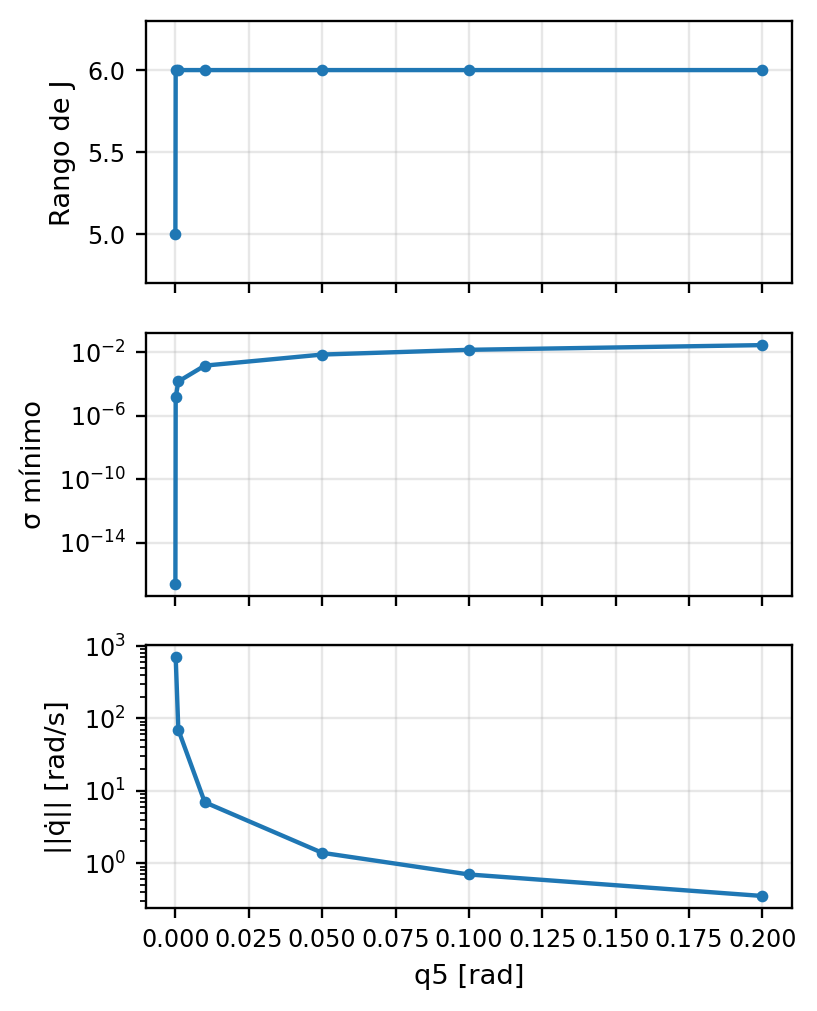
\includegraphics[width=0.91\columnwidth]{figuras/singularidad_muneca.png}
\caption{Experimento computacional independiente de muñeca: (a) rango del Jacobiano, (b) menor valor singular normalizado y (c) amplificación de velocidad articular ante una consigna cartesiana fija. El punto $q_5=0$ es singular y no se invierte $J$.}
\label{fig:sing}
\end{figure}

\subsection{Torque del modelo pedagógico 1R}
Para $t=2.5$\,s, el perfil LSPB 1R entrega $q=1.875$\,rad y $\ddot q=-1$\,rad/s$^2$. Por tanto,
\begin{align}
\tau_I&=0.25(-1)=-0.25\,\mathrm{N\,m},\\
\tau_g&=(1)(9.81)(0.5)\sin(1.875)\nonumber\\
&\simeq4.679791\,\mathrm{N\,m},\\
\tau&\simeq4.429791\,\mathrm{N\,m}.
\end{align}
Durante el crucero, en $t=1.5$\,s, se obtuvo $\tau_I=0$ pero $\tau_g\simeq4.127415$\,N\,m. La Fig.~\ref{fig:tau} presenta los tres componentes temporales. La mayor magnitud de torque observada en la malla temporal de $601$ muestras fue $4.890917$\,N\,m en $t=1.995$\,s: es un \emph{máximo muestreado}, no una garantía de máximo continuo exacto, debido a los cambios abruptos de aceleración del LSPB ideal.

\begin{figure}[!t]
\centering
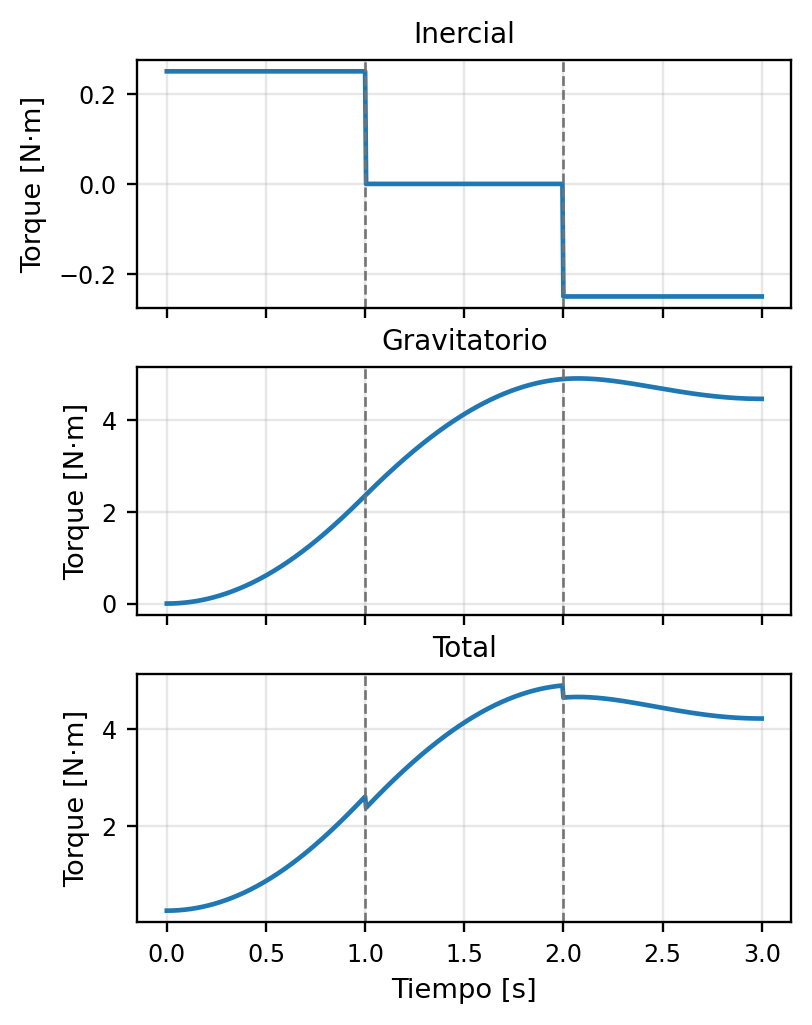
\includegraphics[width=0.91\columnwidth]{figuras/torque_1r.png}
\caption{Torque del modelo reducido 1R de la práctica oficial: componente inercial, componente gravitatoria y suma. Las líneas discontinuas indican las transiciones LSPB en $t=1$ y $2$\,s. Los parámetros son didácticos y no corresponden a inercias ABB.}
\label{fig:tau}
\end{figure}

\section{Discusión}
La selección de una solución de Pieper no concluye la validación del movimiento: es necesario distinguir soluciones matemáticas de configuraciones que satisfacen límites articulares. En el caso de autocontrol, ocho ramas reconstruyeron una misma pose, pero solo dos ramas tuvieron representaciones nominalmente admisibles; la multiplicidad adicional en J6 procede de periodicidad angular. Tampoco la admisibilidad nominal garantiza ausencia de colisiones o factibilidad dinámica.

El Jacobiano cuantifica la relación \emph{instantánea} entre velocidades y revela degradaciones cinemáticas. La aproximación a $q_5=0$ muestra amplificación de velocidades articulares para determinadas demandas cartesianas, pero no implica por sí sola torque infinito. En cambio, la curva $\tau(t)$ del sistema reducido 1R depende de su aceleración y configuración gravitatoria, no de una inversión del Jacobiano del robot 6R. Estos son fenómenos distintos y deben interpretarse separadamente, según la rúbrica oficial \cite{rubricaH2}.

La trayectoria LSPB ideal asegura continuidad de posición y velocidad, pero sus discontinuidades de aceleración pueden originar saltos en la componente inercial del torque. Además, la comparación con los límites nominales ABB de posición y velocidad no equivale a validar colisiones, fuerzas en el TCP, frenado del controlador o límites de aceleración no documentados. Finalmente, los parámetros de inercia, masa y centro de masa del 1R proceden del ejemplo docente y no se atribuyen a los componentes mecánicos del ABB IRB 120.

\section{Reproducibilidad y limitaciones}
El proyecto utiliza módulos Python separados para FK, Pieper, filtrado ABB, LSPB, Jacobiano, singularidades y dinámica 1R, integrados en \texttt{notebooks/hito2\_integracion.ipynb}. El Notebook fue ejecutado por completo en Fedora mediante el kernel \texttt{imt342} y se publicó sin salidas precalculadas, para reconstruir las gráficas al ejecutarlo. La batería de pruebas de regresión reportó \textbf{71 pruebas satisfactorias}. La versión del Notebook quedó registrada en el commit \texttt{e8045e0} de la rama de trabajo \texttt{feature/h2-pieper-lspb}.

\emph{Pendiente académico explícito:} sustituir o ampliar el caso de autocontrol con todas las poses objetivo que asigne el docente, sin alterar los criterios de comprobación. La presente versión no certifica que esos objetivos se hayan procesado. Tampoco constituye una simulación física validada del manipulador ni un controlador apto para ejecución sobre el robot real.

\section{Conclusiones}
Se comprobó computacionalmente la conexión entre una pose cartesiana, las múltiples soluciones analíticas de cinemática inversa, su verificación FK y una trayectoria articular LSPB. El filtrado de límites mostró la importancia de distinguir ramas geométricas de representaciones admisibles. El Jacobiano permitió verificar velocidades cartesianas y exhibir la pérdida de una dimensión de movilidad instantánea en una singularidad de muñeca. Por separado, el modelo dinámico pedagógico 1R reprodujo el valor de torque de la práctica docente y permitió diferenciar los aportes inercial y gravitatorio.

El flujo implementado está validado en el caso de autocontrol; su evaluación completa frente a las poses oficiales y la defensa matemática individual siguen sujetas a las consignas y a la verificación del docente.

\begin{thebibliography}{00}
\bibitem{guiaH2} IMT-342 Robótica, ``Guía Oficial y Rúbrica de Evaluación: Hito 2,'' Universidad Católica Boliviana, material docente, 2026; compilación \textit{S10\_material\_oficial.pdf}, pp. 31--32.
\bibitem{rubricaH2} IMT-342 Robótica, ``Rúbrica Oficial de Evaluación: Hito 2,'' Universidad Católica Boliviana, material docente, 2026; compilación \textit{S10\_material\_oficial.pdf}, pp. 34--36.
\bibitem{practicaS10} IMT-342 Robótica, ``Práctica y solucionario W10-S01,'' Universidad Católica Boliviana, material docente, 2026; compilación \textit{S10\_material\_oficial.pdf}, pp. 13--17.
\bibitem{abbSpec} ABB, \textit{IRB 120: Especificaciones del producto}, documento 3HAC035960-005, rev. W, secs. 1.8.1 y 1.8.3.
\bibitem{abbManual} ABB, \textit{IRB 120: Manual del producto}, documento 3HAC035728-005, rev. W, sec. 2.2.2.
\bibitem{siciliano} B. Siciliano, L. Sciavicco, L. Villani y G. Oriolo, \textit{Robotics: Modelling, Planning and Control}. Springer, 2009.
\end{thebibliography}

\end{document}
